\chapter{Background}
This chapter gives an overview of the necessary background information required for this research. Air quality monitors are explained in a general way with its use, capabilities and sensors. Passive network eavesdropping and private information inference are introduced as this will be the vulnerability exploit in this research. Lastly, this chapter gives an overview of Wi-Fi, Bluetooth, ZigBee and Ethernet that are communication protocols which air quality monitors use to communicate over. \\\\
\section{Air Quality Monitors}
Air quality monitors are used as sensors to collect sensor data from different sources in the air. \cite{GeneralAirQualityMonitor} The IoT devices can store data in different ways. Cloud storing is the most preferred storage solution for IoT devices, but also local servers, internal storage and SD cards can be used to store data from IoT devices and air quality monitors. \cite{AQMBigSource} Displaying data to users of air quality monitors is an important factor to give the user either just information about the indoor quality, or recommendations on how to better the air. \cite{AQMBigSource} The most developed and recent method of doing so, is through an app on the users mobile phone, but also solutions where users can login to a web-site exists. Many air quality monitors also have the functionality of an screen on the device that shows certain values from the sensors. Some of these can also be interactive. \cite{AQMBigSource}
\\\\
Several factors plays a key part when selecting which air quality monitor most suitable for the users needs. Even tough many devices are pre-calibrated when available in store, a test on the specific environment should be done. Considering the different functionality an air quality monitor can have, it is also important to look into transmission range, power consumption and requirements for maintenance. \cite{AQMBigSource} However, the main goal of an air quality monitor is to monitor the air and therefore looking into which kind of sensors the devices have should be a top priority when selecting your device. Air quality monitors can specialize in one measuring unit in the air or have the functionality to measure several air quality factors, such as \(CO_2\), radon, HCHO, noise, VOC, humidity or temperature. The air quality monitors are incorporated in users homes and therefore the appearance of the device will also be a considerable factor for choosing the right device. \cite{IAQMonitorCommunicationReview} 
\\\\
As indoor air quality monitors can be equipped with different features, a brief explanation of some of the features an air quality monitor can sensor is necessary to understand why and how private information can be gathered from these sensors:
\begin{itemize}
    \item \(CO_2\)\\
        Carbon Dioxide, \(CO_2\), is a chemical formula that is made by human or animal combustion, in addition to other larger combustion processes. \cite{CO2} This implicates that the more humans or animals that are in the same indoor environment as the air quality monitor, the higher occurrence of \(CO_2\) will be collected by the sensor and transmitted to the air quality monitors receiver. However, plants and sunlight can bind \(CO_2\) and reduce the amount of \(CO_2\) particles in an indoor environment. Also bad or irregular ventilation will make the \(CO_2\) levels grow.
    \item Radon\\
        Radon is a radioactive gas that is strongly recommended to be measured in Norwegian indoor environments. \cite{Radon} The gas does not have any smell and is invisible and is carcinogenic which makes it an attractive feature to include on the air quality monitor. 
    \item Noise\\
        Noise is an interesting feature of some air quality monitors as it considered a health problem. \cite{Noise} Exposure to loud noises at a small amount of time or long-term noise can both harm peoples health. Especially when considering a work environment where workers need to concentrate, noises over long periods of time can result in hearing difficulties or problems communicating. As many work from home and we use a lot of time in our home, the problem is also applicable here. 
    \item VOC\\
        Volatile organic compounds, VOC, is a collective term for any combination of carbon, with the exception of carbon monoxide, carbon dioxide, carbonic acid, metallic carbides or carbonates and ammonium carbonate. \cite{VOC} These harmful compounds can be found in gases from building materials or smoking, cleaning articles, painting or cooking to mention some. TVOC is a term for defining the total amount of VOCs. The amount of VOC in the indoor environment can be simply reduced by ensuring fresh air and using kitchen fans to prevent the articles from circulating the indoor air to be breathed by users. \cite{RecommendedIAQ}
     \item HCHO\\
        HCHO is the chemical formula for formaldehyde which is a gas that can cause severe health effects. \cite{HCHO} The gas contains a strong odor and is flammable when it has room temperature, but is colorless. People can be exposed to HCHO from several different sources such as manufacture wood products, building materials, fertilizers, cigarettes, paint, glue or even medicines and cosmetics. Formaldehyde is classified as a VOC.
    \item Humidity\\
        Humidity is calculated from the ratio between water vapor in the air compared to the maximum amount of water vapor possible in the air if the air was saturated. \cite{RecommendedIAQ} Even tough humans can endure high variations in humidity, very low percentages of humidity can result in health problems such as irritated eyes, dry skin or dry moucus membranes. The humidity is correlated by temperature, which means that variations in temperature can effect the humidity percentage. Normal home behaviour that can affect the humidity is taking a shower, drying clothes and cooking. 
    \item Temperature\\
        Temperature is a measure unit for how hot or cold the environment is and is measured using a thermometer. Temperature is the most commonly used unit for how comfortable humans feel. Temperature can affect humans health on both ends of the scale. A too high temperature can result in lack of energy and sleepiness and a too low temperature can result in reduced muscle function or heighten symptoms of rheumatism. \cite{Temp}
\end{itemize}


\\\\
As air quality monitors can be a part of a smart home care system, it can also include in a Wireless Body Area Network (WBAN) to sensor the indoor environment. Therefore, it can be vulnerable to several security threats and attacks by malicious actors. \cite{AttackstoAQMs} 
\\\\

\subsection{Private Information Inference}
Considering the amount of information an air quality monitor can collect about an individual or a smart home, privacy leakage is a vulnerability. \cite{SecPrivSmartCity} When malicious attackers tries to gather sensitive information about an individual user or group of users, a privacy attack is carried out. \cite{CyberEntitySecInIoT} The aim of the attacker is then to target the confidentiality of the user, while gathering information such as location, preferences, personal behaviour or similar private information.

\subsection{Passive Network Eavesdropping}
Eavesdropping network communication can either be passive or active. When an attacker conducts an active eavesdropping attack on a target, the data in the communication link is both inferred and modified. \cite{Eavesdropping} While in a passive network eavesdropping attack, the eavesdropper does not modify any data on the link, but simply aims to gather data transmitted without changing the communication. The overall goal of eavesdropping is therefore often to access private information that are being sent on the channel. That can be anything from credentials to secret messages, or as in this research, private information about users and their habits. \cite{Eavesdropping} Since the communication is not effected by a passive network eavesdropping attack, the attacker does not need to be as careful in disguising itself as in an active attack.  
\\
There are security measures to implement to reduce the chance of being eavesdropped, both actively and passively. Since an eavesdroppers goal is to listen in on the communication, encrypting the traffic is an effective way to make it harder to conduct an eavesdropping attack. Also, covert channels that hide the identity of the communicating parties can be used to prevent the eavesdropper from finding the right communication channel to eavesdrop. \cite{Eavesdropping}
\\\\
\section{Communication Protocols}
Air Quality Monitors send their sensoring data to remote server for storing and analyzing the data. As they exists with different functionality and specifications, their communication protocols differs, like other groups of IoT devices. \cite{AQMBigSource} Wi-Fi is the most preferred protocol with Bluetooth and Zigbee following. \cite{saini2020indoor} As this thesis is delimited to air quality monitor devices that uses Wi-Fi, Bluetooth, Zigbee or wired communication trough Ethernet as communication protocols, the next subsections will elaborate on these protocols and specifications to be used further in this thesis through testing and analysis. 

\subsection{IEEE 802.11 - Wi-Fi}
Wireless Fidelity (Wi-Fi) \cite{WiFiAlliance} is one of the worlds most used technology for communicating and is defined, developed and standarized by WiFi Alliance. \cite{WiFiAlliance} Wi-Fi is based on the standard IEEE 802.11 Wireless LAN set by IEEE Standard for Information Technology. \cite{WifiStandard} The transmission range for Wi-Fi is up to 100 meters and it uses 5-60GHz in the frequency band. \cite{IAQMonitorCommunicationReview}
\\\\

\\\\
\subsection{Bluetooth}
Bluetooth is a communication protocol based on the IEEE 802.15.1 standard set out by the IEEE Standard for Information Technology. The frequency band for Bluetooth is 2.4GHz and the transmission rate is up to 10 meters, which is relatively shorter compared to Wi-Fi. \cite{IAQMonitorCommunicationReview} Due to the transmission range of Bluetooth it is mainly used for short-range communication, which can be very suitable for air quality monitors configured to transmit data to a hub or nearby other wireless devices, such as mobile phones. Since many IoT devices are designed to communicate in short ranges within a house, Bluetooth Low Energy (BLE) was introduced as a version suitable for this specific communication. \cite{SecurityofCommunicationProt} As the name says, BLE has a reduced power consumption, compared to WiFi, and is therefore often chosen as communication protocol for IoT devices. 
\\\\
When a Bluetooth device are starting a data exchange with another device, a paring process is established between the two communicating parties \cite{BluetoothCommunication}. The parties are one slave and one master, where the master is usually the device with the highest resources. For example an IoT devices, such as AQMs, as slaves and mobile phones as master. They find each other by listening to an advertising channel where devices waiting to connect are broadcasting messages. When connected, the parties change to another channel to exchange data called a Piconet. This channel is divided into time-slots where each party has its slots for communicating. The channel has the masters MAC address as the piconet address. This functionality makes it harder to eavesdrop as communication is not demand-based, but based on time slots. 

Bluetooth packets contains the following fields, also shown in figure X

\begin{itemize}
    \item \textbf{Channel Access Code:} Identifies the communication on the specific physical channel. 
    \item \textbf{Packet Header:} Includes source and destination for the packet and are used to route the packet. Also includes link control protocol. 
    \item \textbf{Guard and Sync:} Only used for enhanced data rate packets where guard time and synchronization is necessary before the payload is examined.
    \item \textbf{Payload Header:} Includes logic link identifier used for further routing and the size of the following payload.
    \item \textbf{Payload Body:} The field where the actual data transmitted relies. 
    \item \textbf{Message Integrity Check:} Only used with AES-CCM encryption.
    \item \textbf{Cyclic Redundancy Check:} Detects if packets have errors. 
\end{itemize}


\subsection{ZigBee}
ZigBee is also a popular choice for communication protocol when it comes to IoT devices. The protocol is based on the IEEE 802.15.4 standard set by IEEE Standard for Information Technology, but is developed by the Zigbee alliance \cite{ZigBeeStandard} \cite{ZigbeeAlliance}. ZigBee uses the same frequency band as Bluetooth, 2.4GHz, but also supports the frequencies 915MHz and 868MHz, and does obtain a longer transmission rate up to 20 meters. \cite{IAQMonitorCommunicationReview} The 2,4GHz frequency band contains 16 different channels for communication. \cite{ZigbeeOverview} Some of the advantages of ZigBee, and especially in IoT devices, are low data rate, low cost and long battery life. 
\\\\
ZigBee MAC-frame consists of three main parts, header, payload and footer, and four header fields, see figure \ref{ZigBeePic} \cite{ZigBeBasics}:
\begin{itemize}
    \item \textbf{Frame Control:} Contains information about the frame type, addressing fields and additional control flags.
    \item \textbf{Sequence Number:} Beacon Sequence Number
    \item \textbf{Addressing Fields:} Addresses for source and destination
    \item \textbf{Auxiliary Security HDR:} Optional and used for security processing
    \item \textbf{MAC Payload:}  The payload of the frame
    \item \textbf{MAC Footer (MFR):} Data verification with frame check sequence
\end{itemize}

\begin{figure}[h]
    \centering
    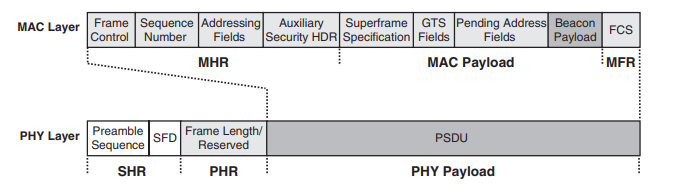
\includegraphics[width=0.5\textwidth]{figures/Zigbee.png}
    \caption{ZigBee MAC frame}
    \label{ZigbeePic}
\end{figure}

\subsection{Ethernet}

\subsection{Comparison of the different communication protocols}
In Table \ref{CommunicationProtocolsComparison} a comparison of the different communication protocols that will be used during tests in this thesis and their specifications are presented. \\
\begin{table}[!hbtp]
\begin{tabular}{||c | c | c | c ||} 
 \hline
 Communication Protocol & Frequency Band & Transmission Range & Power consumption\\ [0.5ex]
 \hline\hline
 Wi-Fi & 5-60GHz & 100m & High\\ 
 Bluetooth & 2.4GHz & 10m & Low\\
 ZigBee & 2.4GHz & 20m & Low \\
 Ethernet & Very variable & 100m & Plugged\\ [1ex] 
 \hline
\end{tabular}
\caption{Communication Protocols Comparison}
\label{CommunicationProtocolsComparison}
\end{table}